\documentclass{beamer}
%\usetheme{Warsaw}
%\usecolortheme{orchid}
\usetheme{metropolis}
\usepackage[polish]{babel}
\usepackage[utf8]{inputenc}
\usepackage{amsfonts}
\usepackage{indentfirst}
\usepackage[T1]{fontenc}
\usepackage{amsmath}
\usepackage{hyperref}
\usepackage{graphicx}
\usepackage{graphics}
\usepackage{subcaption}

\title{
Zaawansowane metody uczenia maszynowego
}
\subtitle{
Projekt 1
}
\author{
Mikołaj Małkiński
}
\institute{
Politechnika Warszawska \\
Wydział Matematyki i Nauk Informacyjnych
}
\date{\today}

\begin{document}

    \maketitle

    \begin{frame}{Spis treści}
        \setbeamertemplate{section in toc}[sections numbered]
        \tableofcontents[hideallsubsections]
    \end{frame}

    \section{Przygotowanie danych}

    \begin{frame}
        \frametitle{Brakujące dane}
        \begin{figure}
            \centering
            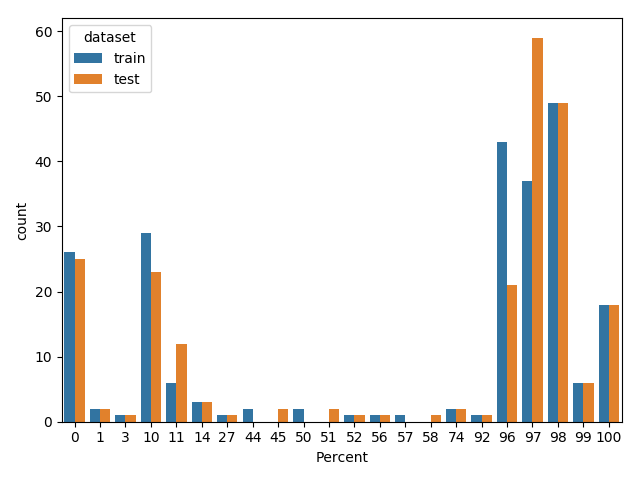
\includegraphics[width=0.8\linewidth]{../images/missing-data.png}
            \caption{Liczba kolumn posiadających dany procent brakujących danych z podziałem na zbiór treningowy i testowy}
            \label{fig:missing-data}
        \end{figure}
    \end{frame}

    \begin{frame}
        \frametitle{Brakujące dane - rozwiązanie}
        \begin{itemize}
            \item Usunięcie kolumn które mają więcej niż 90\% braków
            \item Kolumny numeryczne - wypełnienie medianą
            \item Kolumny kategoryczne - dodanie nowej kategorii: \textit{unknown}
        \end{itemize}
    \end{frame}

    \begin{frame}
        \frametitle{Unikalność danych - rozwiązanie}
        \begin{itemize}
            \item Usunięcie kolumn kategorycznych z 1 unikalną wartością
            \item Usunięcie kolumn kategorycznych z ponad 100 unikalnymi wartościami
            \item (Opcjonalnie) - potraktowanie kolumn numerycznych mających mało unikalnych danych jako kategoryczne
        \end{itemize}
    \end{frame}

    \begin{frame}
        \frametitle{Przekształcenie kolumn kategorycznych - One-hot encoding}
        \begin{figure}
            \centering
            \begin{subfigure}{0.4\textwidth}
                \centering
                \begin{tabular}{c}
                    Var42 \\
                    \hline
                    foo \\
                    bar \\
                    bar \\
                    foo \\
                    foo \\
                \end{tabular}
                \caption{Przed}
            \end{subfigure}
            \begin{subfigure}{0.4\textwidth}
                \centering
                \begin{tabular}{c|c}
                    Var42\_foo & Var42\_bar \\
                    \hline
                    1 & 0 \\
                    0 & 1 \\
                    0 & 1 \\
                    1 & 0 \\
                    1 & 0 \\
                \end{tabular}
                \caption{Po}
            \end{subfigure}
            \caption{One-hot encoding na kolumnie posiadającej 2 różne wartości}
            \label{fig:one-hot-encoding}
        \end{figure}
    \end{frame}

    \section{Analiza danych}

    \begin{frame}
        \frametitle{Porównawcza analiza danych}
        \begin{figure}
            \centering
            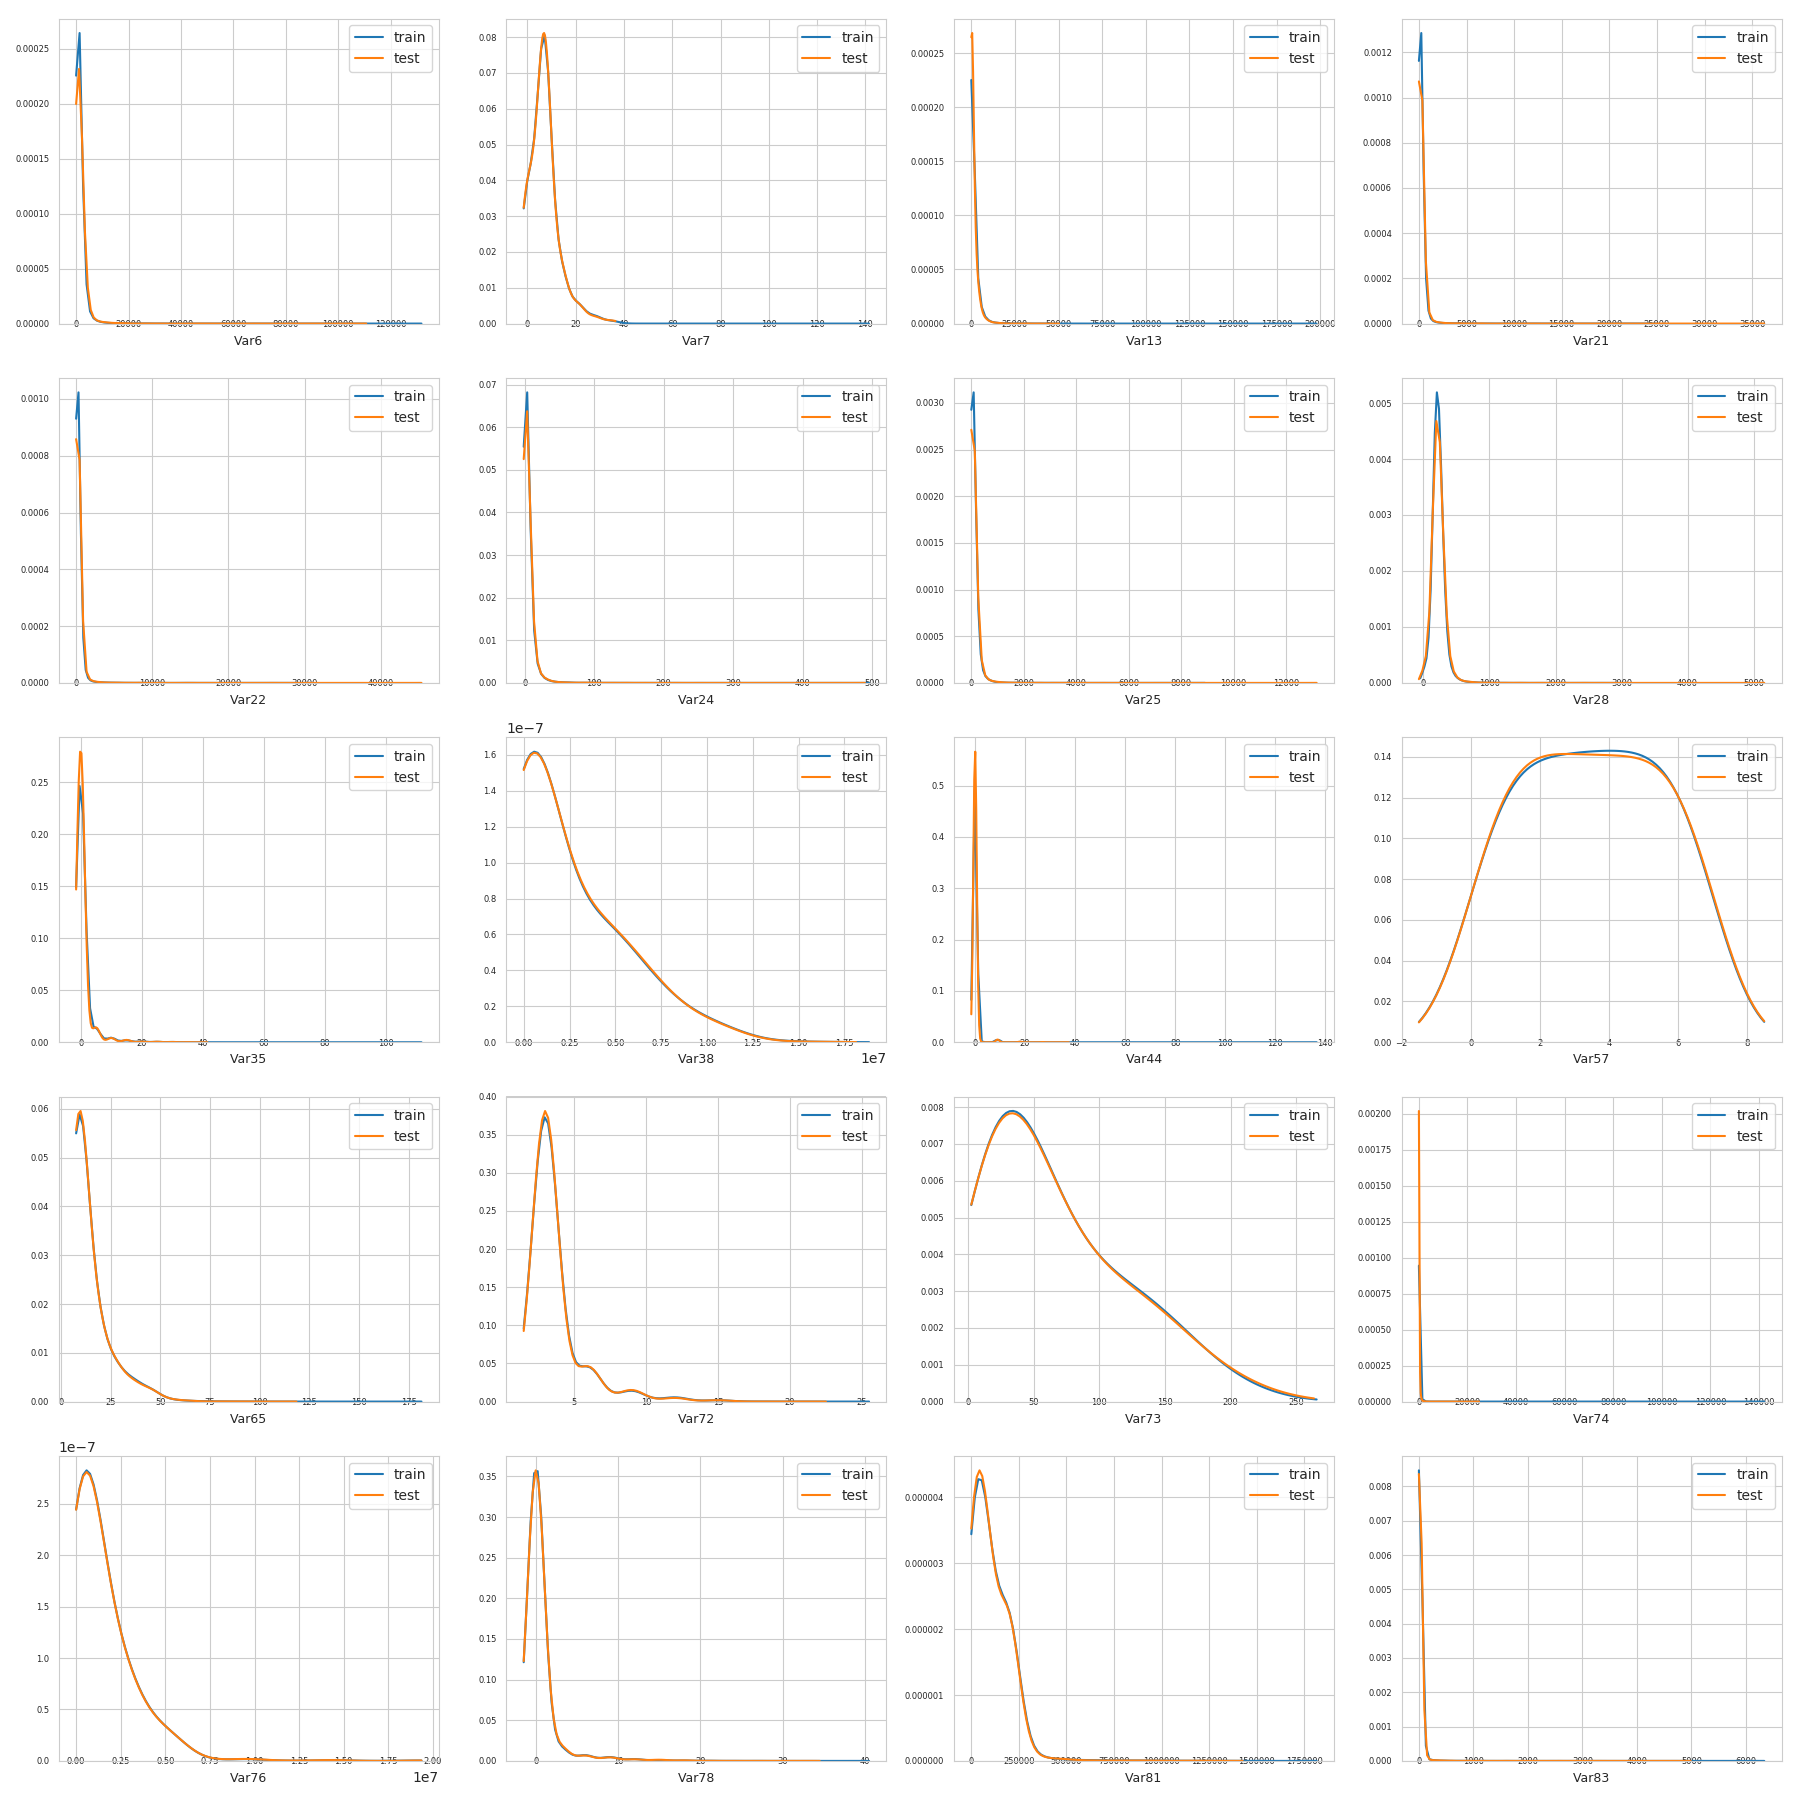
\includegraphics[width=0.7\linewidth]{../images/feature-distribution-0-20-train-test.png}
            \caption{Porównanie rozkładów cech ze względu na zbiór}
            \label{fig:feature-distribution-0-20-train-test}
        \end{figure}
    \end{frame}

    \begin{frame}
        \frametitle{Porównawcza analiza danych}
        \begin{figure}
            \centering
            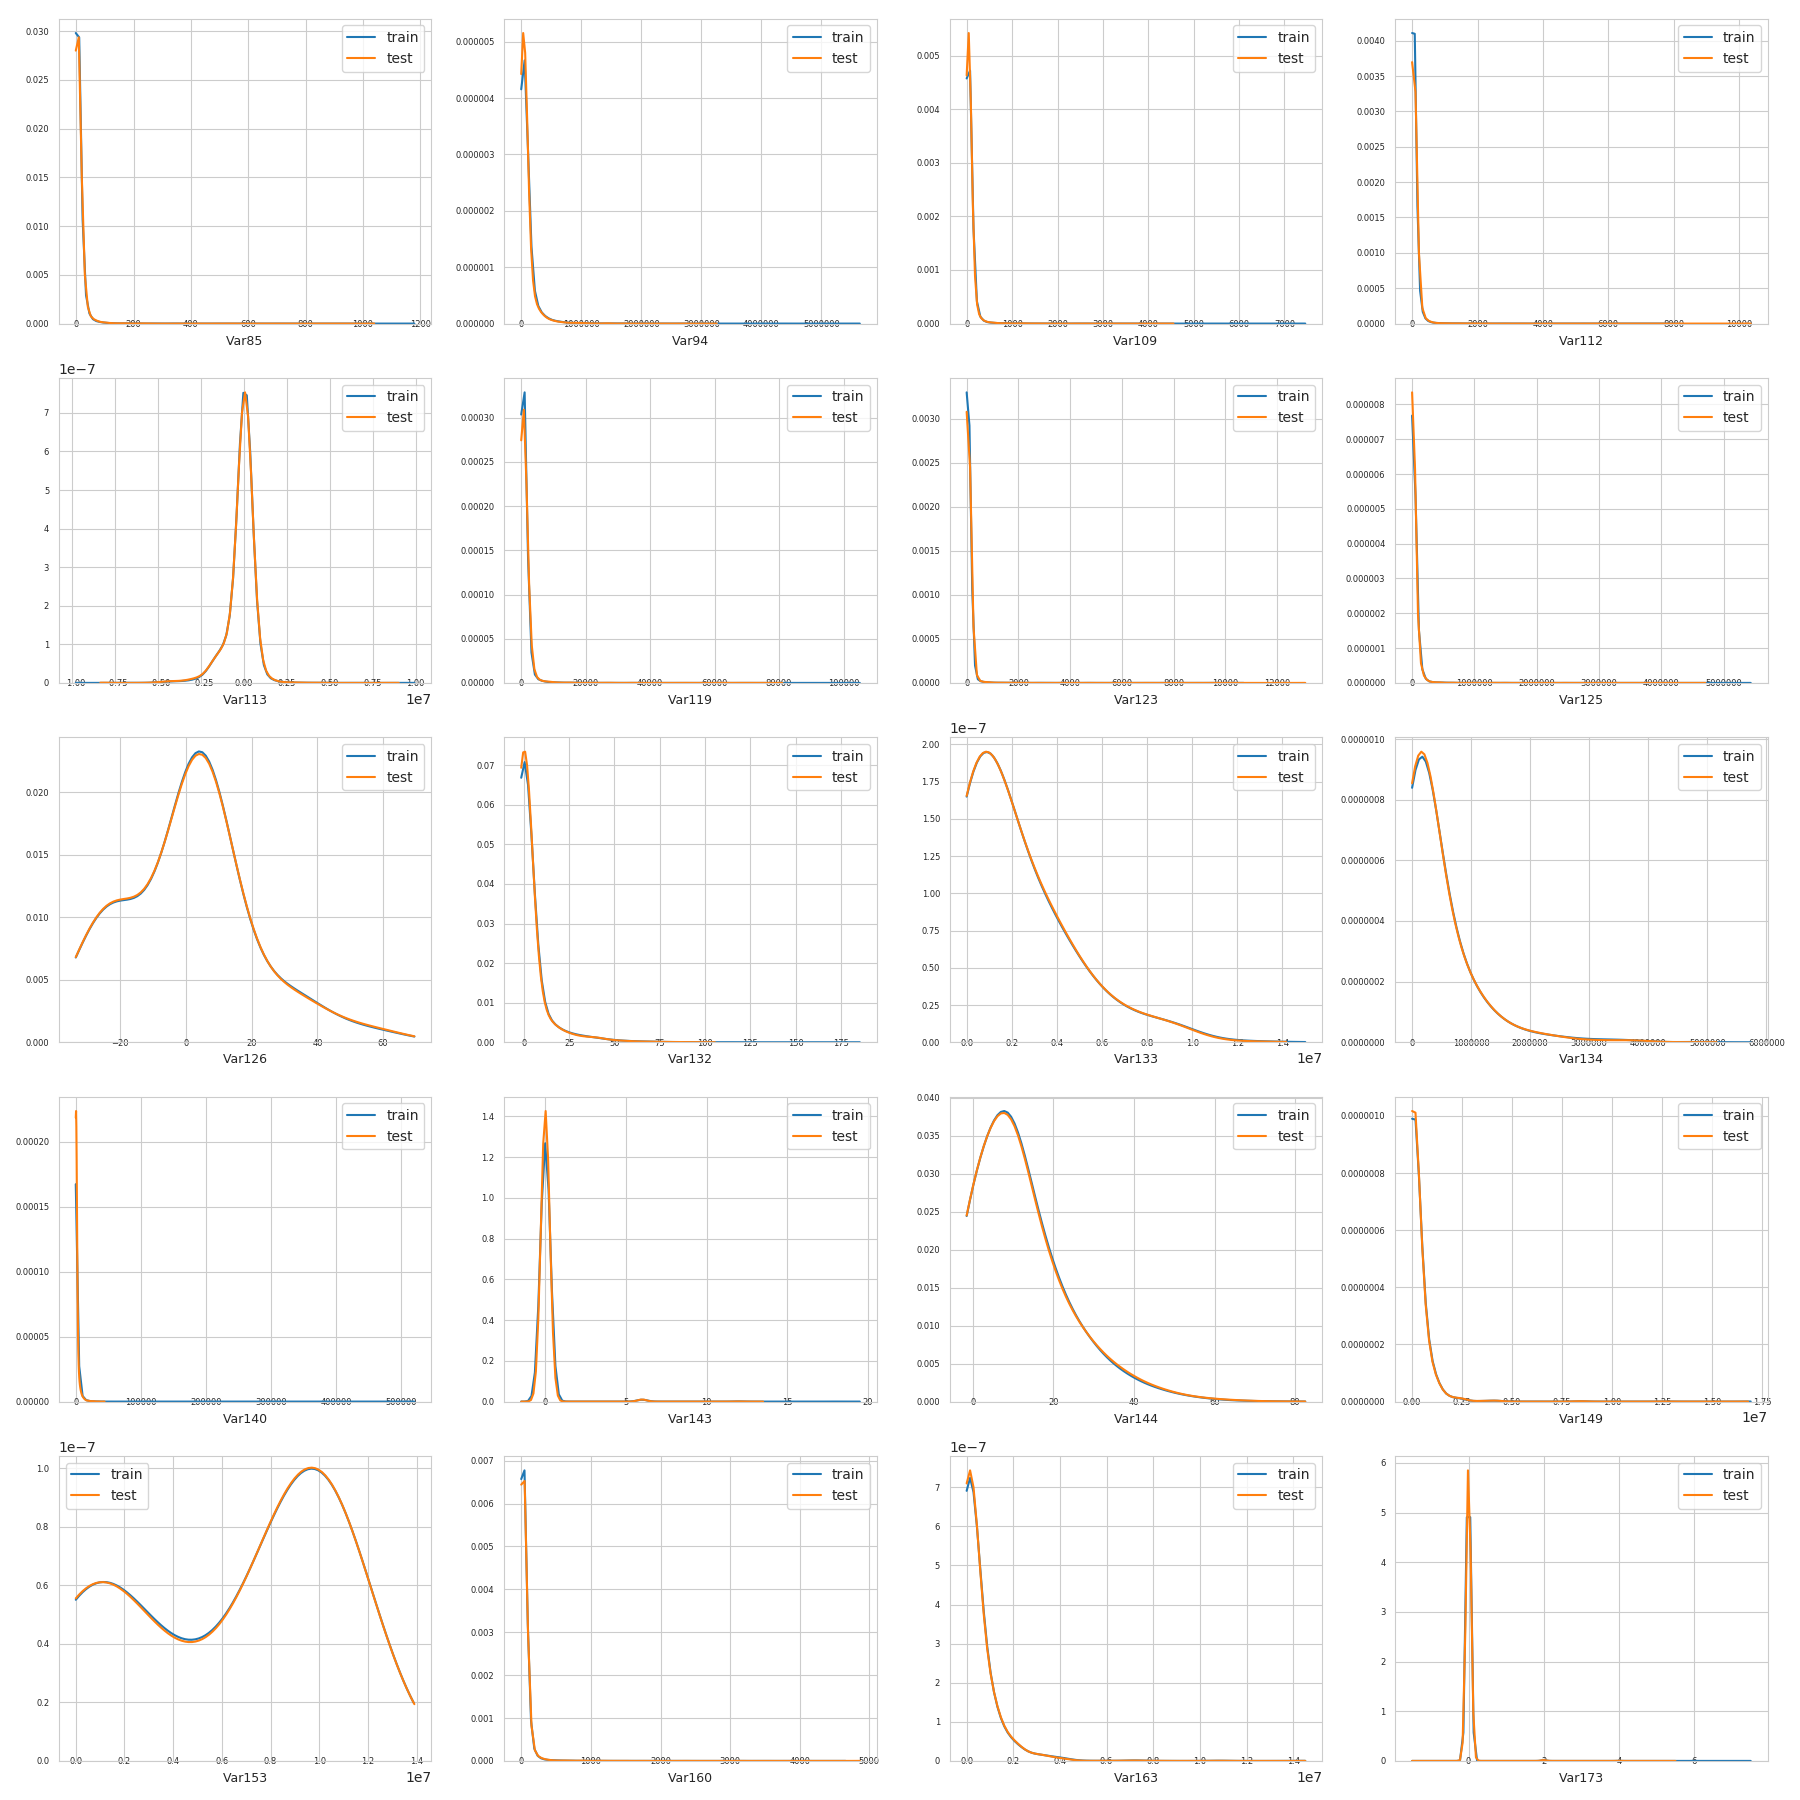
\includegraphics[width=0.7\linewidth]{../images/feature-distribution-20-40-train-test.png}
            \caption{Porównanie rozkładów cech ze względu na zbiór}
            \label{fig:feature-distribution-20-40-train-test}
        \end{figure}
    \end{frame}

    \begin{frame}
        \frametitle{Porównawcza analiza danych}
        \begin{figure}
            \centering
            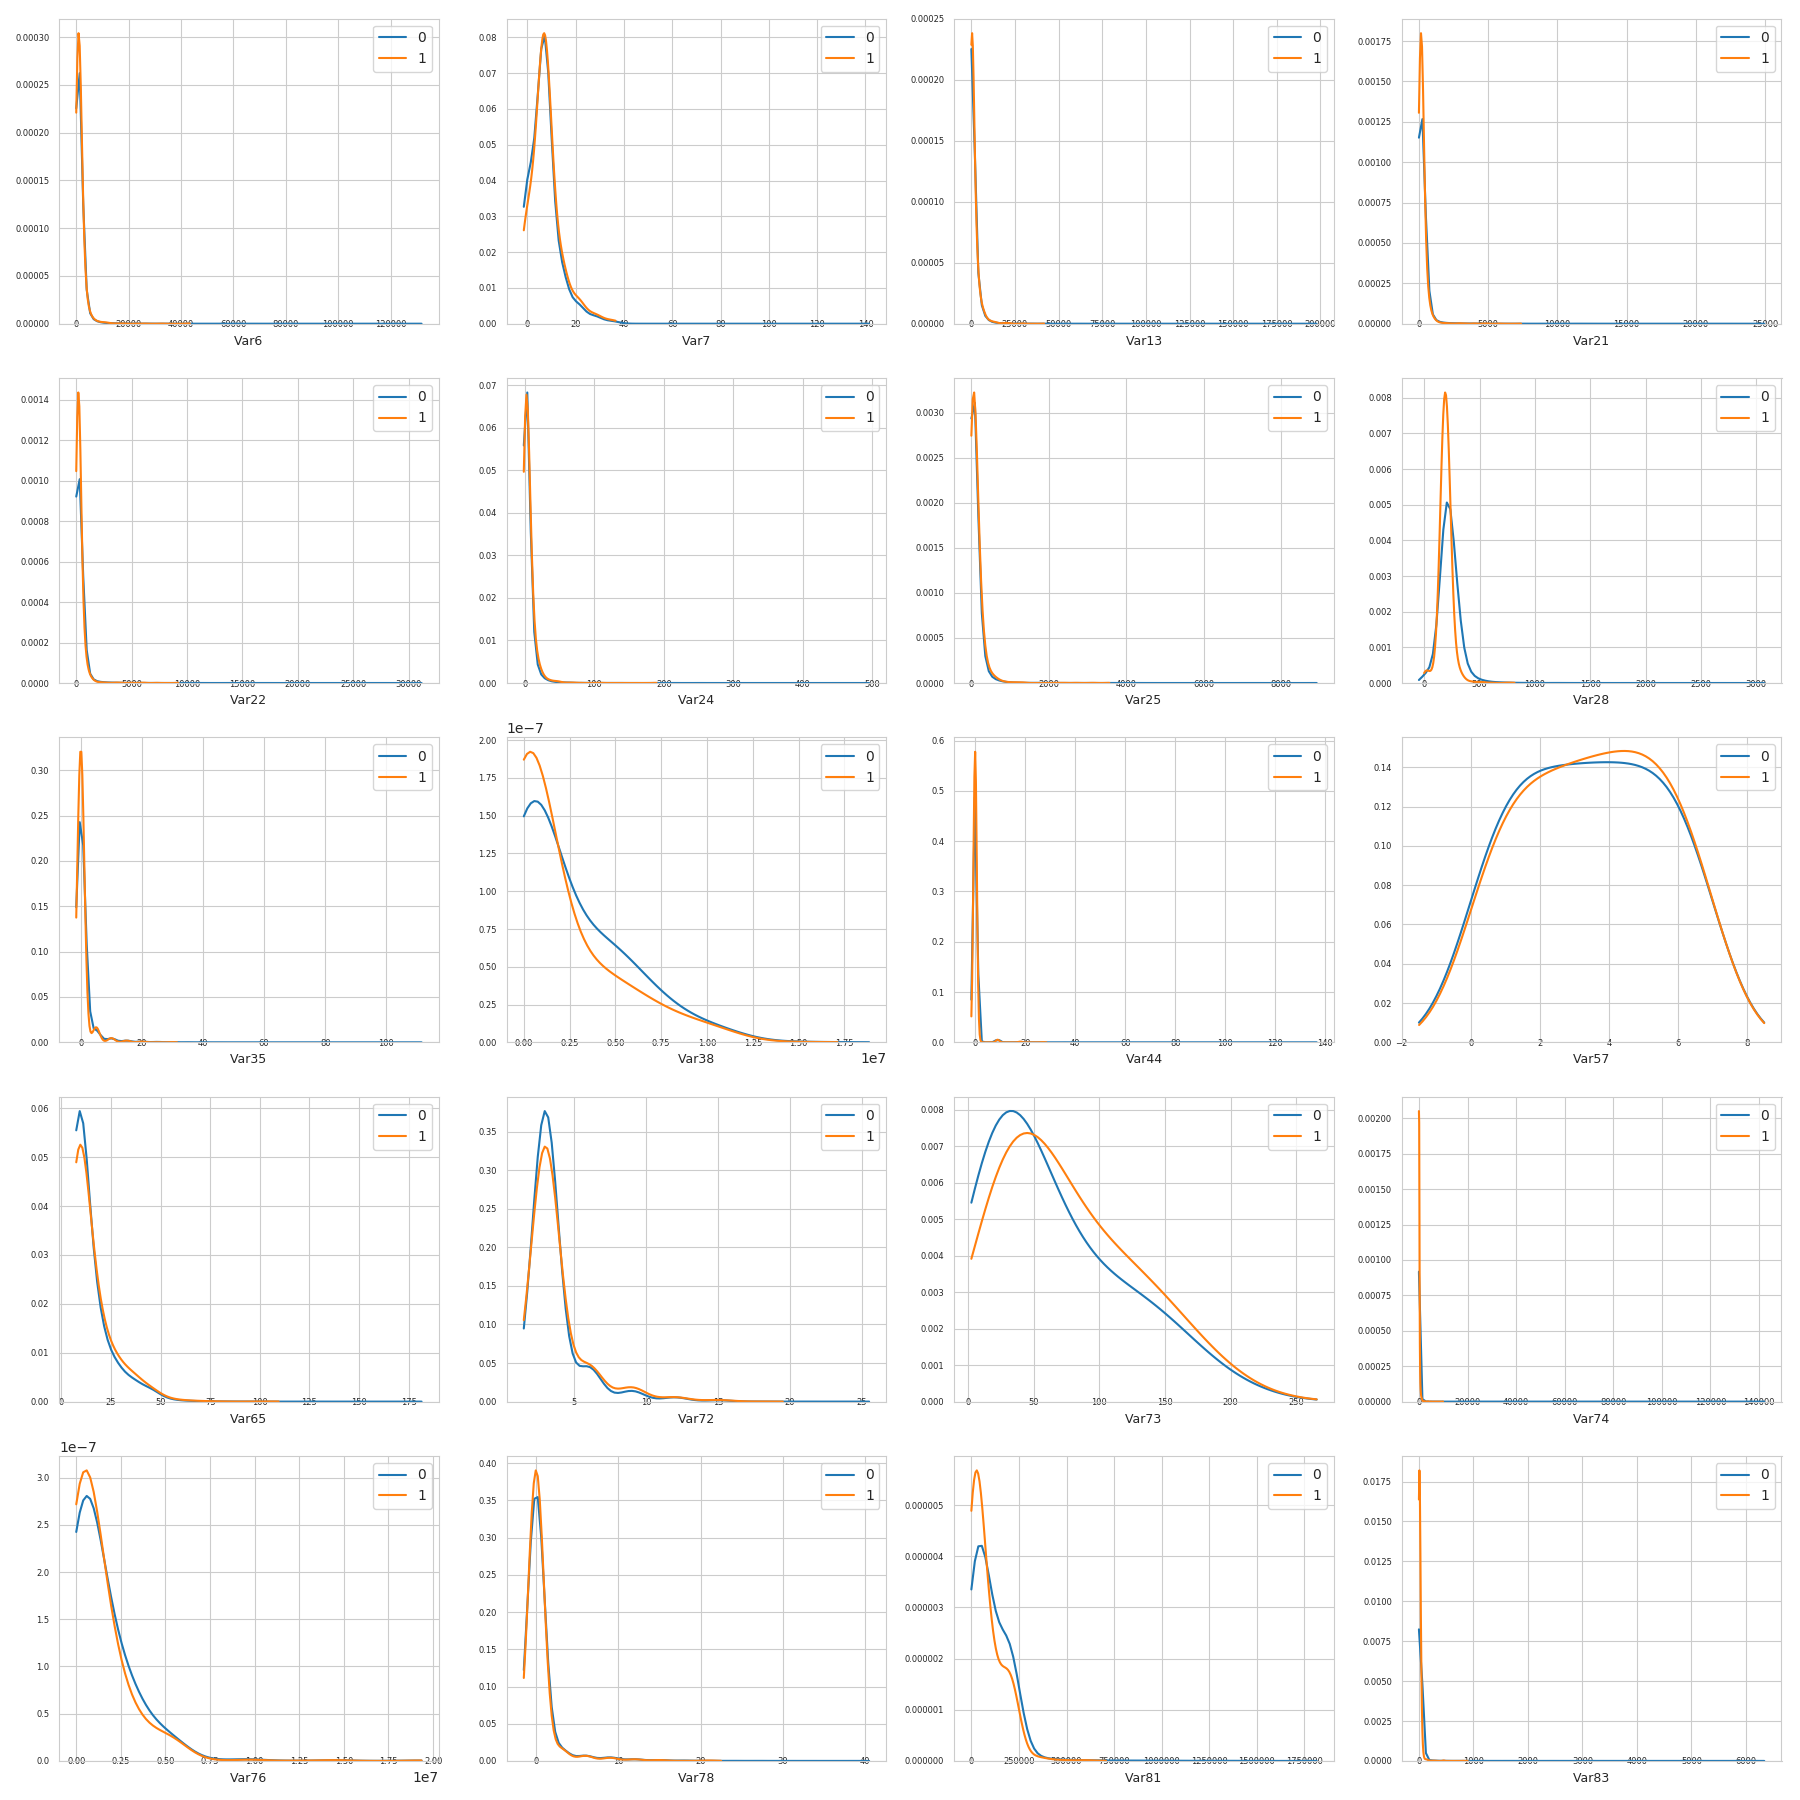
\includegraphics[width=0.7\linewidth]{../images/feature-distribution-0-20.png}
            \caption{Porównanie rozkładów cech ze względu na klasę}
            \label{fig:feature-distribution-0-20}
        \end{figure}
    \end{frame}

    \begin{frame}
        \frametitle{Porównawcza analiza danych}
        \begin{figure}
            \centering
            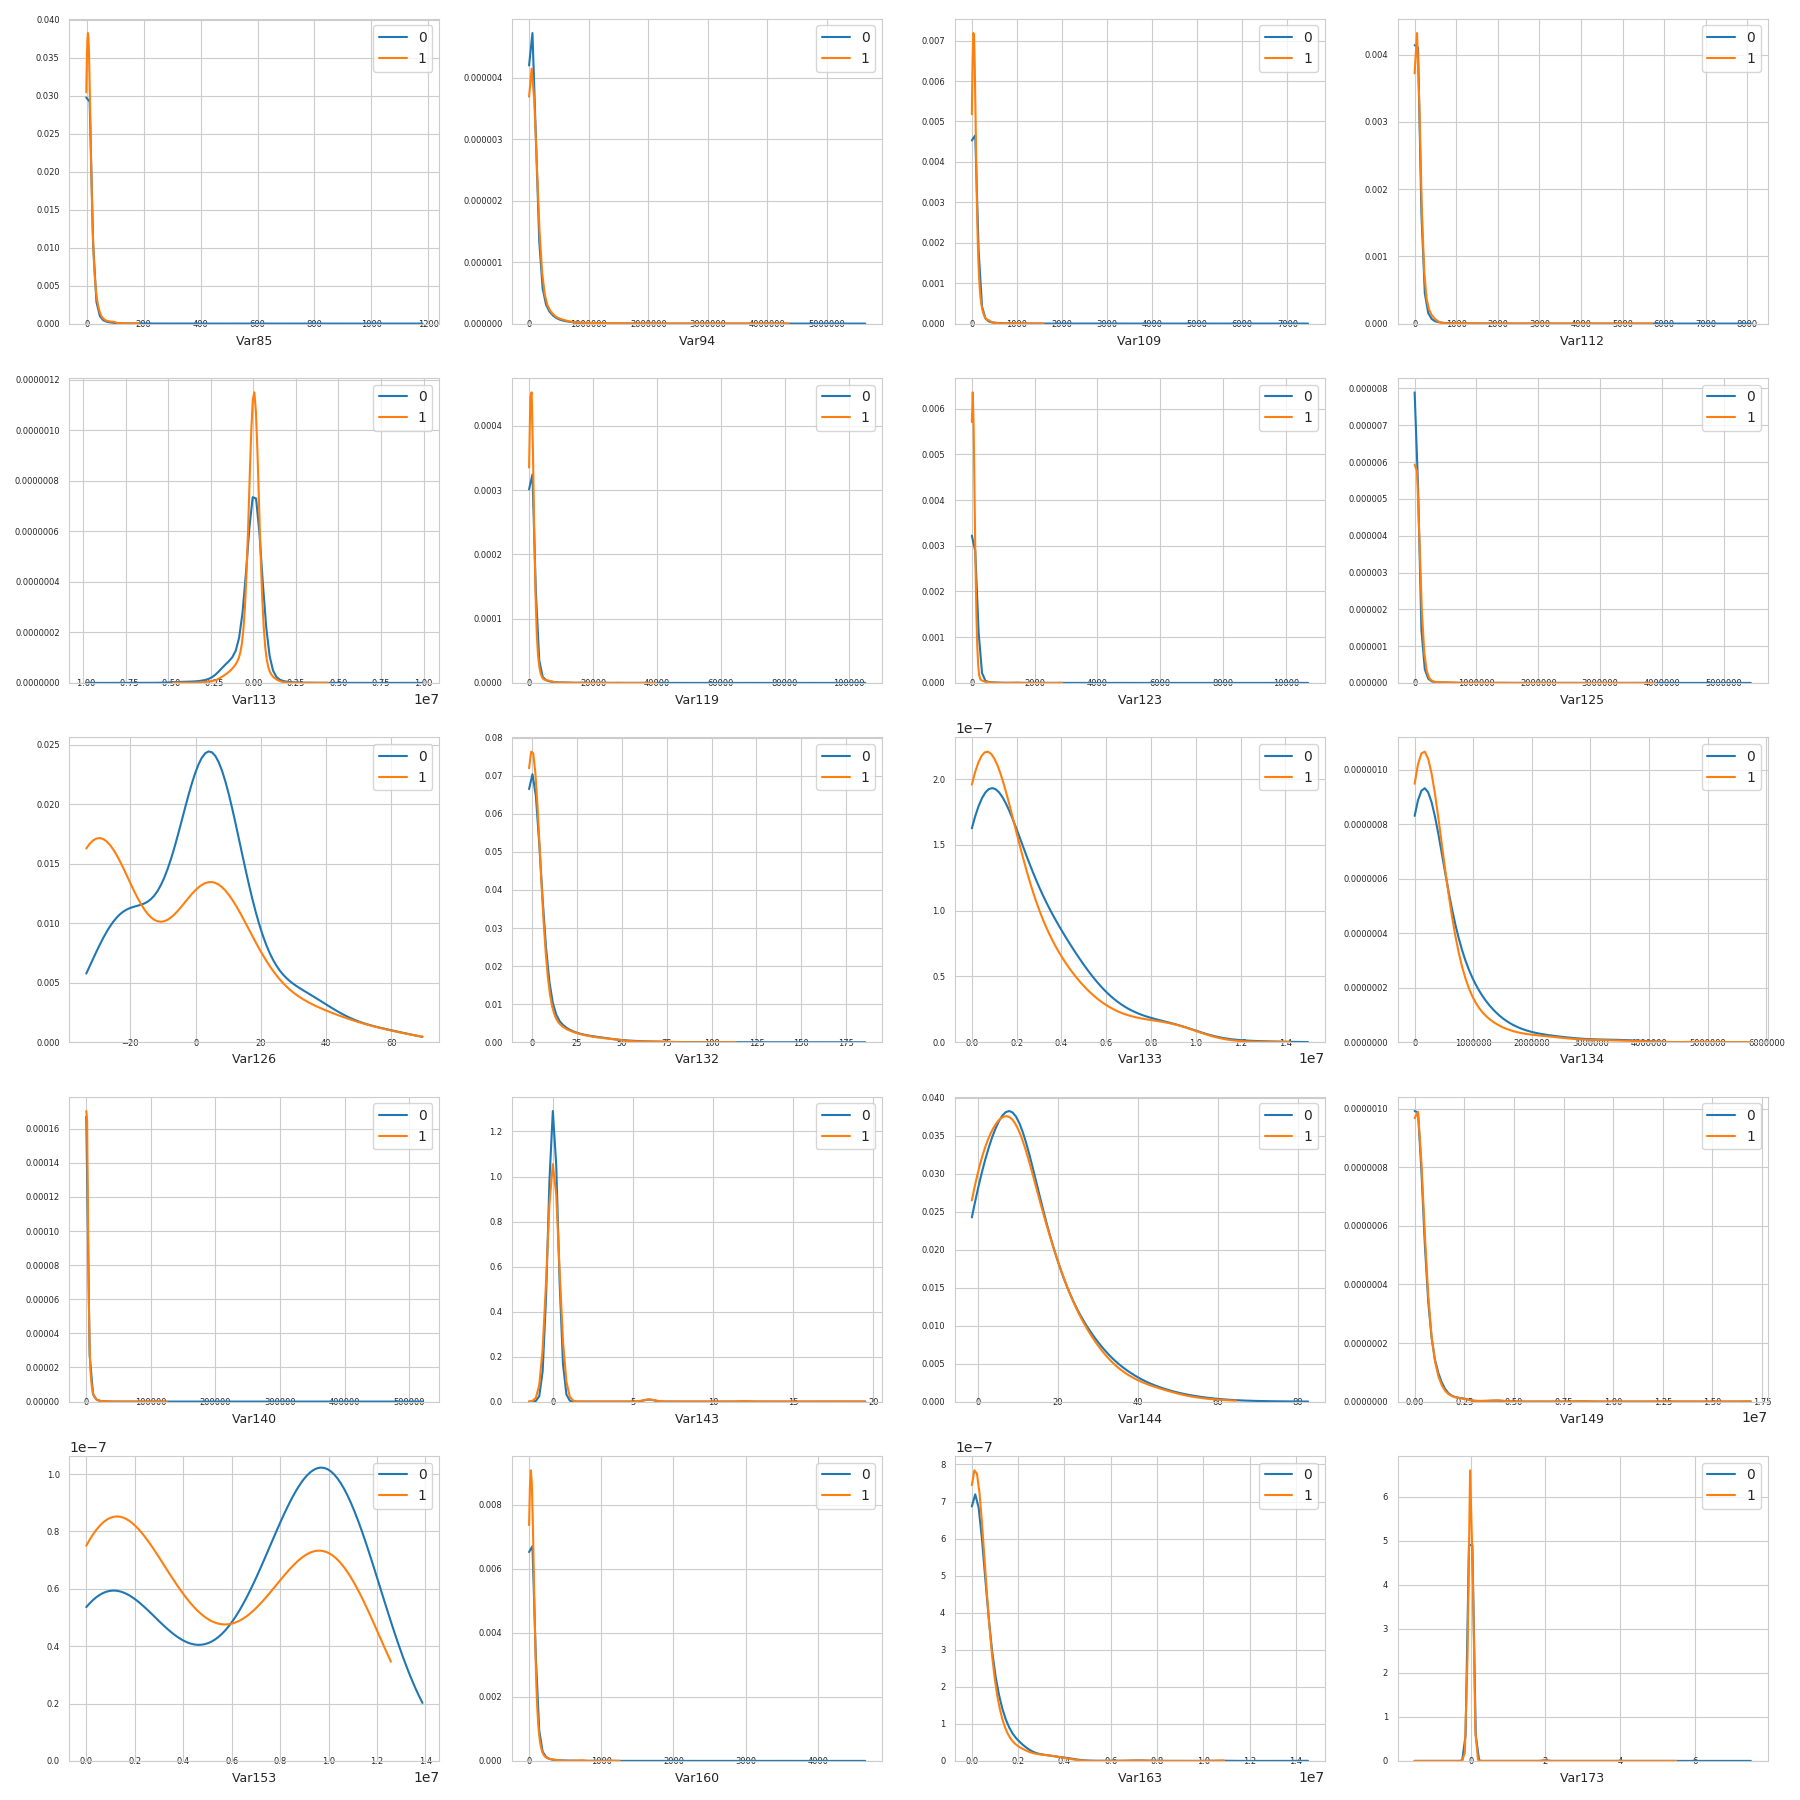
\includegraphics[width=0.7\linewidth]{../images/feature-distribution-20-40.png}
            \caption{Porównanie rozkładów cech ze względu na klasę}
            \label{fig:feature-distribution-20-40}
        \end{figure}
    \end{frame}

    \section{Podstawowe klasyfikatory}

    \begin{frame}
        \frametitle{Podstawowe klasyfikatory}
        \begin{itemize}
            \item XGBoost
            \item XGBoost balanced
            \item LightGBM
            \item LightGBM balanced
            \item CatBoost
            \item CatBoost balanced
            \item AdaBoost
            \item GradientBoosting
            \item RandomForest
            \item BalancedRandomForest
            \item ExtraTrees
        \end{itemize}
    \end{frame}

    \begin{frame}
        \frametitle{Podstawowe klasyfikatory - krzywe ROC}
        \begin{figure}
            \centering
            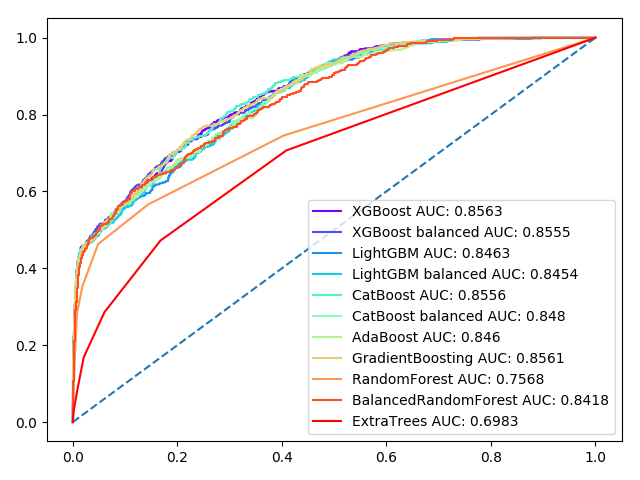
\includegraphics[width=0.8\linewidth]{../images/roc-comparison.png}
            \caption{Porównanie krzywych ROC podstawowych modeli klasyfikacyjnych}
            \label{fig:roc-comparison}
        \end{figure}
    \end{frame}

    \begin{frame}
        \frametitle{Podstawowe klasyfikatory - rezultaty}
        \resizebo
        \begin{table}
            \begin{tabular}{l|*{3}{c}}
                & AUC & Dokładność & Precyzja@10 \\
                \hline
                XGBoost & \textbf{0.8563} & \textbf{0.9516} & \textbf{0.3600} \\
                XGBoost balanced & 0.8555 & 0.7742 & 0.3588 \\
                LightGBM & 0.8463 & 0.9508 & 0.3575 \\
                LightGBM balanced & 0.8454 & 0.8654 & 0.3488 \\
                CatBoost & 0.8556 & 0.9514 & 0.3500 \\
                CatBoost balanced & 0.8480 & 0.8450 & 0.3563 \\
                AdaBoost & 0.8460 & 0.9505 & 0.3550 \\
                GradientBoosting & 0.8561 & 0.9510 & 0.3588 \\
                RandomForest & 0.7568 & 0.9404 & 0.3250 \\
                BalancedRandomForest & 0.8418 & 0.7332 & 0.3575 \\
                ExtraTrees & 0.6983 & 0.9328 & 0.2162 \\
            \end{tabular}
            \caption{Metryki podstawowych modeli klasyfikacyjnych}
            \label{tab:score-comparison1}
        \end{table}
    \end{frame}

    \begin{frame}
        \frametitle{Podstawowe klasyfikatory - rezultaty}
        \resizebo
        \begin{table}
            \begin{tabular}{l|*{3}{c}}
                & F1 & Precyzja & Czułość \\
                \hline
                XGBoost & \textbf{0.5442} & \textbf{0.7524} & 0.4262 \\
                XGBoost balanced & 0.3043 & 0.1923 & 0.7288 \\
                LightGBM & 0.5310 & 0.7483 & 0.4114 \\
                LightGBM balanced & 0.3631 & 0.2672 & 0.5664 \\
                CatBoost & 0.5418 & 0.7492 & 0.4244 \\
                CatBoost balanced & 0.3467 & 0.2426 & 0.6070 \\
                AdaBoost & 0.5308 & 0.7417 & 0.4133 \\
                GradientBoosting & 0.5410 & 0.7404 & 0.4262 \\
                RandomForest & 0.2891 & 0.7519 & 0.1790 \\
                BalancedRandomForest & 0.2707 & 0.1661 & \textbf{0.7306} \\
                ExtraTrees & 0.0561 & 0.5714 & 0.0295 \\
            \end{tabular}
            \caption{Metryki podstawowych modeli klasyfikacyjnych}
            \label{tab:score-comparison2}
        \end{table}
    \end{frame}

    \section{Próby poprawienia wyników}

    \begin{frame}
        \frametitle{Metody balansowania klas}
        \begin{itemize}
            \item Zmniejszenie ilości obserwacji z klasy 0
            \item Zwiększenie ilości obserwacji z klasy 1
            \item Dodanie sztucznych obserwacji z klasy 1 używając techinki SMOTE
        \end{itemize}
    \end{frame}

    \begin{frame}
        \frametitle{Wybór cech}
        \begin{itemize}
            \item Przygotowany zbiór danych posiadał 470 różnych kolumn
            \item Wytrenowanie modeli XGBoost, LightGBM oraz CatBoost
            \item Wybranie 30 najbardziej istotnych cech dla każdego modelu
            \item Połączenie zbiorów dało 57 najważniejszych cech
        \end{itemize}
    \end{frame}

    \section{Optymalizacja najlepszego modelu}

    \begin{frame}
        \frametitle{Dobór hiperparametrów}
        Aby dobrać hiperparametry, użyto 3-krotnej kroswalidacji oraz kierowano się jak największą wartością metryki precyzja@10.
        Metody:
        \begin{itemize}
            \item Random search
            \item Grid search
        \end{itemize}
        Hiperparametry:
        \begin{itemize}
            \item stosunek klas
            \item maksymalna głębokość drzew wchodzących w skład komitetu (base learners)
            \item współczynnik uczenia
            \item liczba członków komitetu
            \item współczynniki próbkowania
        \end{itemize}
    \end{frame}

    \begin{frame}
        \frametitle{Ostateczna ewaluacja - krzywe ROC}
        \begin{figure}[!h]
            \centering
            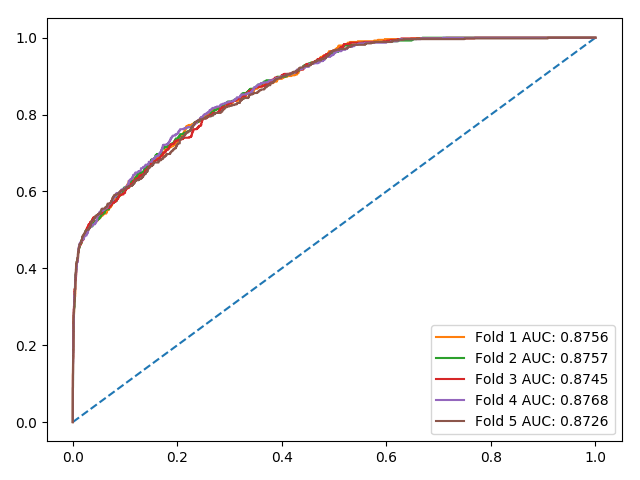
\includegraphics[width=0.8\textwidth]{../images/xgb-roc-comparison.png}
            \caption{Porównanie krzywych ROC zoptymalizowanego modelu XGBoost używając kroswalidacji}
            \label{fig:xgb-roc-comparison}
        \end{figure}
    \end{frame}

    \begin{frame}
        \frametitle{Ostateczna ewaluacja - metryki}
        \begin{table}
            \begin{tabular}{l|*{3}{c}}
                & AUC & Dokładność & Precyzja@10 \\
                \hline
                Próba 1 & 0.8605 & 0.7779 & 0.4000 \\
                Próba 2 & 0.8757 & 0.7960 & 0.4263 \\
                Próba 3 & 0.8702 & 0.7770 & 0.4075 \\
                Próba 4 & 0.8621 & 0.7758 & 0.3987 \\
                Próba 5 & 0.8569 & 0.7755 & 0.3812 \\
                \hline
                Średnia & 0.8651 & 0.7804 & \textbf{0.4027} \\
            \end{tabular}
            \caption{Metryki zoptymalizowanego modelu XGBoost używając kroswalidacji}
            \label{tab:xgb-score-comparison1}
        \end{table}
    \end{frame}

    \begin{frame}
        \frametitle{Ostateczna ewaluacja - metryki}
        \begin{table}
            \begin{tabular}{l|*{3}{c}}
                & F1 & Precyzja & Czułość \\
                \hline
                Próba 1 & 0.3210 & 0.2071 & 0.7131 \\
                Próba 2 & 0.3625 & 0.2395 & 0.7448 \\
                Próba 3 & 0.3283 & 0.2099 & 0.7530 \\
                Próba 4 & 0.3215 & 0.2055 & 0.7378 \\
                Próba 5 & 0.3087 & 0.1971 & 0.7110 \\
                \hline
                Średnia & 0.3284 & 0.2118 & 0.7319 \\
            \end{tabular}
            \caption{Metryki zoptymalizowanego modelu XGBoost używając kroswalidacji}
            \label{tab:xgb-score-comparison2}
        \end{table}
    \end{frame}

    \section{Podsumowanie}

    \begin{frame}
        \frametitle{Podsumowanie}
        \begin{itemize}
            \item Osiągnięty wynik (40.27\%) znacznie odbiega od idealnego (70\%)
            \item Wyniki zastosowanych modeli klasyfikacyjnych były do siebie zbliżone
            \item Optymalizacja hiperparametrów dla wybranego modelu (XGBoost) przyniosła poprawę jego jakości zbliżoną do 4\%
            \item Główną przeszkodą było silne zanonimizowanie zbioru danych
        \end{itemize}
    \end{frame}

    \begin{frame}[standout]
        \centering
        Dziękuję za uwagę
    \end{frame}

\end{document}
